\documentclass[a4paper,ngerman,12pt]{scrartcl}

\usepackage[utf8]{inputenc}
%\usepackage[ansinew]{inputenc}

\usepackage[ngerman]{babel}

\usepackage{amsmath,amsthm,amssymb,stmaryrd,color,graphicx}
\usepackage{setspace}
\usepackage{bussproofs}
\usepackage{array}
\usepackage{comment}

\usepackage{enumitem}

\usepackage{units}

\usepackage[protrusion=true,expansion=true]{microtype}

\usepackage{lmodern}

\usepackage{hyperref}
\usepackage{cleveref}
\usepackage{wrapfig}

\newcommand{\RR}{\mathbb{R}}
\newcommand{\CC}{\mathbb{C}}
\newcommand{\ZZ}{\mathbb{Z}}
\newcommand{\NN}{\mathbb{N}}
\newcommand{\QQ}{\mathbb{Q}}

\setlength\parskip{\medskipamount}
\setlength\parindent{0pt}

\theoremstyle{definition}
\newtheorem{defn}{Definition}[]
\newtheorem{axiom}[defn]{Axiom}
\newtheorem{bsp}[defn]{Beispiel}

\theoremstyle{plain}
\newtheorem{prop}[defn]{Proposition}
\newtheorem{motto}[defn]{Motto}
\newtheorem{wunder}[defn]{Wunder}
\newtheorem{ueberlegung}[defn]{Überlegung}
\newtheorem{lemma}[defn]{Lemma}
\newtheorem{kor}[defn]{Korollar}
\newtheorem{hilfsaussage}[defn]{Hilfsaussage}
\newtheorem{satz}[defn]{Satz}

\theoremstyle{remark}
\newtheorem{bem}[defn]{Bemerkung}
\newtheorem{aufg}[defn]{Aufgabe}

\newlength{\aufgabenskip}
\setlength{\aufgabenskip}{1.4em}
\newcounter{aufgabennummer}
\newenvironment{aufgabe}[1]{
  \addtocounter{aufgabennummer}{1}
  \textbf{Aufgabe \theaufgabennummer.} \emph{#1} \par
}{\vspace{\aufgabenskip}}

\clubpenalty=10000
\widowpenalty=10000
\displaywidowpenalty=10000

\setlength\unitlength{1cm}

\usepackage{tikz}

\RequirePackage{geometry}
\geometry{textwidth=16.0cm,textheight=24.5cm,footskip=1.5cm}

\begin{document}

\begin{picture}(0,0)
  \put(0,-0.5){%
    
\includegraphics[scale=0.1]{logo-ifm}
  }
  \put(14.0,-3.5){%
    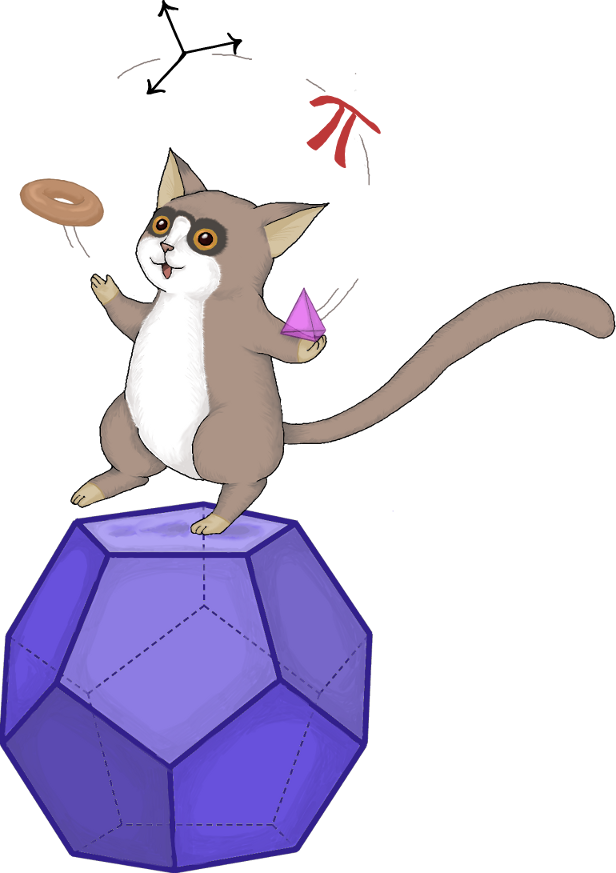
\includegraphics[scale=0.17]{cover}
  }
\end{picture} 

\vspace{6em}


\section*{Fraktale Dimensionen - Lösungshinweise}

Dieses Skript enthält Lösungs\emph{hinweise} zum letzten Korrespondenzbrief. Manchmal sind dies schon die kompletten Lösungen der Aufgaben, meistens sind es aber nur einige Hinweise, die dir dabei helfen sollen, auch die Aufgaben lösen zu können, bei denen du bisher nicht weiter gekommen bist. Wenn du noch weitere Fragen zu den Aufgaben hast, kannst du uns diese weiterhin gerne per E-Mail stellen.

Wenn du uns bereits deine eigenen Lösungsversuche geschickt hast (oder noch schicken wirst - das ist selbstverständlich immer noch möglich), dann versuchen wir natürlich auch dir mit unseren Korrekturen beim Verständnis der Aufgaben zu helfen. Es lohnt sich also uns deine Lösungen zu senden :-)

\begin{aufgabe}{}
	Mit der gleichen Überlegung wie für den zweiten Schritt erhält man:
	\begin{itemize}
		\item Nach $3$ Schritten eine Länge von $\left(\frac{4}{3}\right)^3\cdot l = \frac{4}{3}\cdot\frac{4}{3}\cdot\frac{4}{3}\cdot l = \frac{64}{27}l \approx 2,37 \cdot l$
		\item Nach $5$ Schritten eine Länge von $\left(\frac{4}{3}\right)^5\cdot l = \frac{4}{3}\cdot\frac{4}{3}\cdot\frac{4}{3}\cdot\frac{4}{3}\cdot\frac{4}{3}\cdot l  \approx 4,21 \cdot l$
		\item Nach $n$ Schritten eine Länge von $\left(\frac{4}{3}\right)^n\cdot l$
	\end{itemize}
\end{aufgabe}

\begin{aufgabe}{Wo ist der Schnee?}
	\begin{wrapfigure}{r}{.4\textwidth}\vspace{-1cm}
		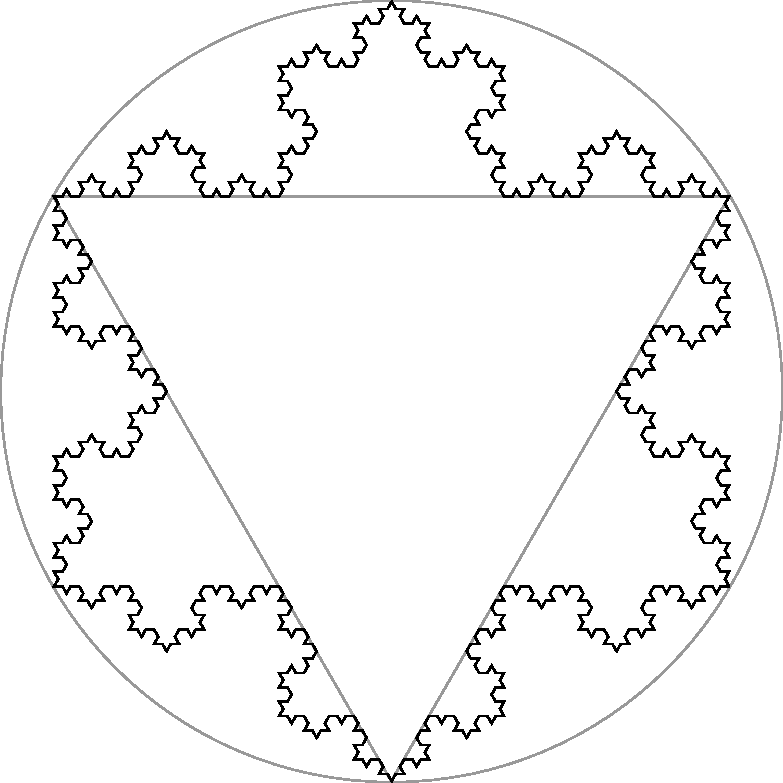
\includegraphics[width=.4\textwidth]{Bilder/Schneeflocke-Umkreis.pdf}
	\end{wrapfigure}

Der Umfang der Kochschen Schneeflocke ist offenbar dreimal so lang wie die Länge einer der drei Kochschen Kurven, aus denen sie besteht. Da deren Länge aber schon unendlich ist, ist natürlich auch der Umfang der Kochschen Schneeflocke unendlich.

Interessanterweise ist aber der Flächeninhalt der Kochschen Schneeflocke trotzdem endlich. Zum Beispiel kann man sich leicht überlegen, dass der Flächeninhalt kleiner sein muss als der des Umkreises des ursprünglichen Dreiecks - und der ist sicher endlich.

% Wenn man den Flächeninhalt exakt bestimmen möchte...  \[1 + \frac{1}{3} + \left(\frac{1}{3}\right)^2 + \dots = ???\]
\end{aufgabe}

\newpage

\begin{aufgabe}{Wie oft?} \label{aufgabe:Wie_oft}
\begin{center}
	\renewcommand{\arraystretch}{2}
	\begin{tabular}{l||c|c|c|c}
		Streckfaktor:& $2$-fach & $3$-fach & $4$-fach & $9$-fach \\\hline\hline
		Strecke      & $2$-mal	& $3$-mal  & $4$-fach & $9$-fach \\\hline
		Dreieck      & $4$-mal  & $9$-mal  & $16$-fach & $81$-fach \\\hline
		Quadrat      & $4$-mal  & $9$-mal  & $16$-fach & $81$-fach  \\\hline
		Würfel       & $8$-mal  & $27$-mal  & $64$-fach & $729$-fach  \\\hline
		Kochschee Kurve & ---   & $4$-mal  & ---      & $16$-mal  \\      	
	\end{tabular}
\end{center}
\end{aufgabe}

\begin{aufgabe}{Potenzen und Dimensionen}
\begin{center}
	\renewcommand{\arraystretch}{2}
	\begin{tabular}{l||c|c|c|c}
				      & $2$ & $3$ & $4$ & $9$ \\\hline\hline
		$\boxed{\phantom{1}}^1$  & $2^1=2$	& $3^1=3$ & $4^1=4$  & $9^1=9$ \\\hline
		$\boxed{\phantom{1}}^2$  & $2^2=4$	& $3^2=9$ & $4^2=16$ & $9^2=81$\\\hline
		$\boxed{\phantom{1}}^3$  & $2^3=8$	& $3^3=27$ & $4^3=64$ & $9^3=729$ \\\hline
		$\boxed{\phantom{1}}^{1,262}$  & $2,398$ & $4,001$ & $5,752$ & $16,005$     	
	\end{tabular}
\end{center}

Es fällt auf (in den ersten drei Zeilen): Streckt man ein $d$-dimensionales Objekt um den Faktor $k$, so passt das ursprüngliche genau $k^d$-mal in das neue. Das passt also genau zu unserer Definition 2 aus dem Korrespondenzbrief.

Damit diese Regel auch für die Kochsche Kurve gilt, müssen wir diese anscheinend als (ungefähr) $1,262$-dimensionales Objekt bezeichnen.

\end{aufgabe}

\begin{aufgabe}{}
	\begin{minipage}{\textwidth}
		\begin{minipage}[t]{0.7\textwidth}
			\renewcommand{\arraystretch}{2}
			\begin{center}
				\begin{tabular}{l||c|c}
				Streckfaktor:& $2$-fach & $4$-fach \\\hline\hline
				Fraktal-Baum & $3$-mal & $9$-mal \\	
			\end{tabular}
			\end{center}
		\end{minipage}
		\begin{minipage}[t]{0.2\textwidth}\vspace{-1.5cm}
			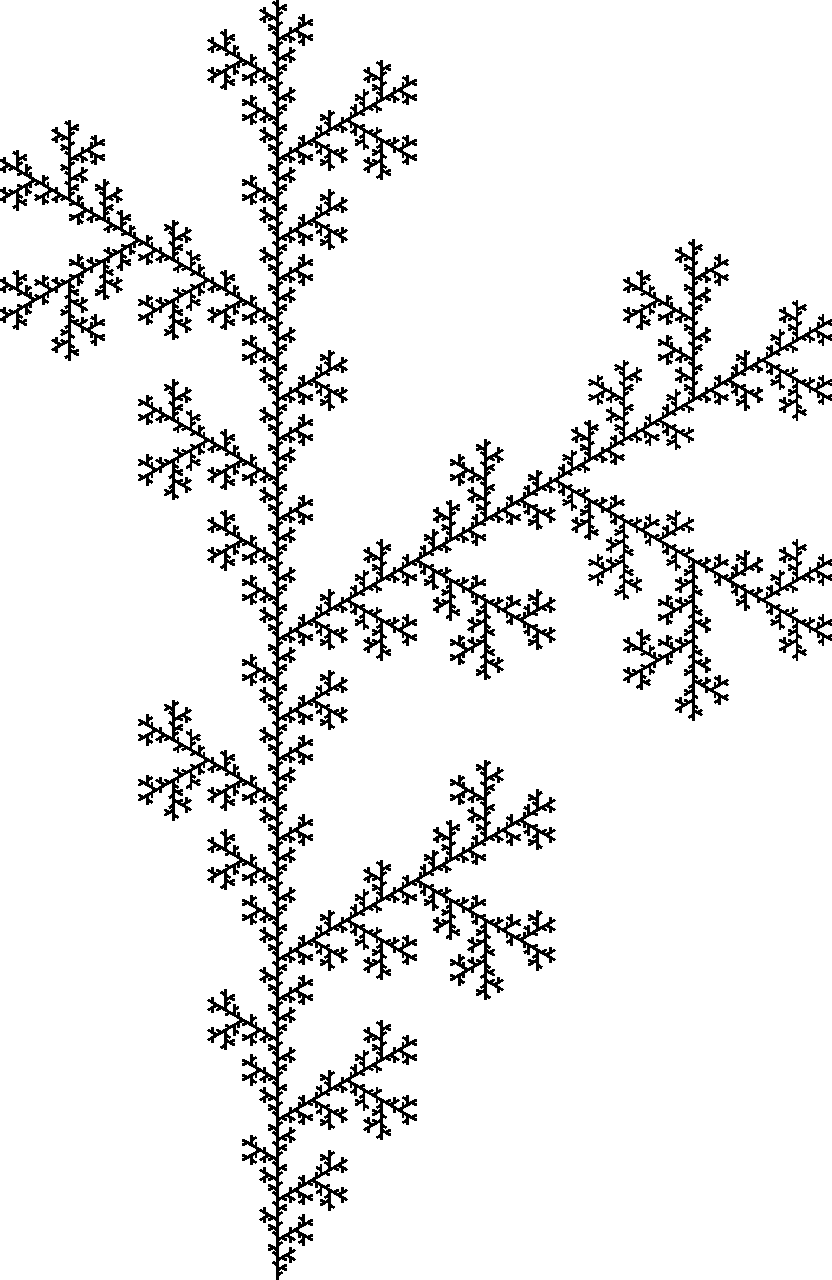
\includegraphics[width=0.5\textwidth]{Bilder/Baum.pdf}
		\end{minipage}
	\end{minipage}
	
	Vergleichst du die obige Tabelle mit der aus Aufgabe 3, so siehst du dass die Dimension des Fraktalbaumes zwischen der einer Strecke und der eines Dreiecks liegt - also zwischen $1$ und $2$. Eine exakte Berechnung liefert: $d \approx 1,585$.
\end{aufgabe}

\newpage
\begin{aufgabe}{}\label{aufgabe:Sierpinski-Flaeche}
	\begin{center}
		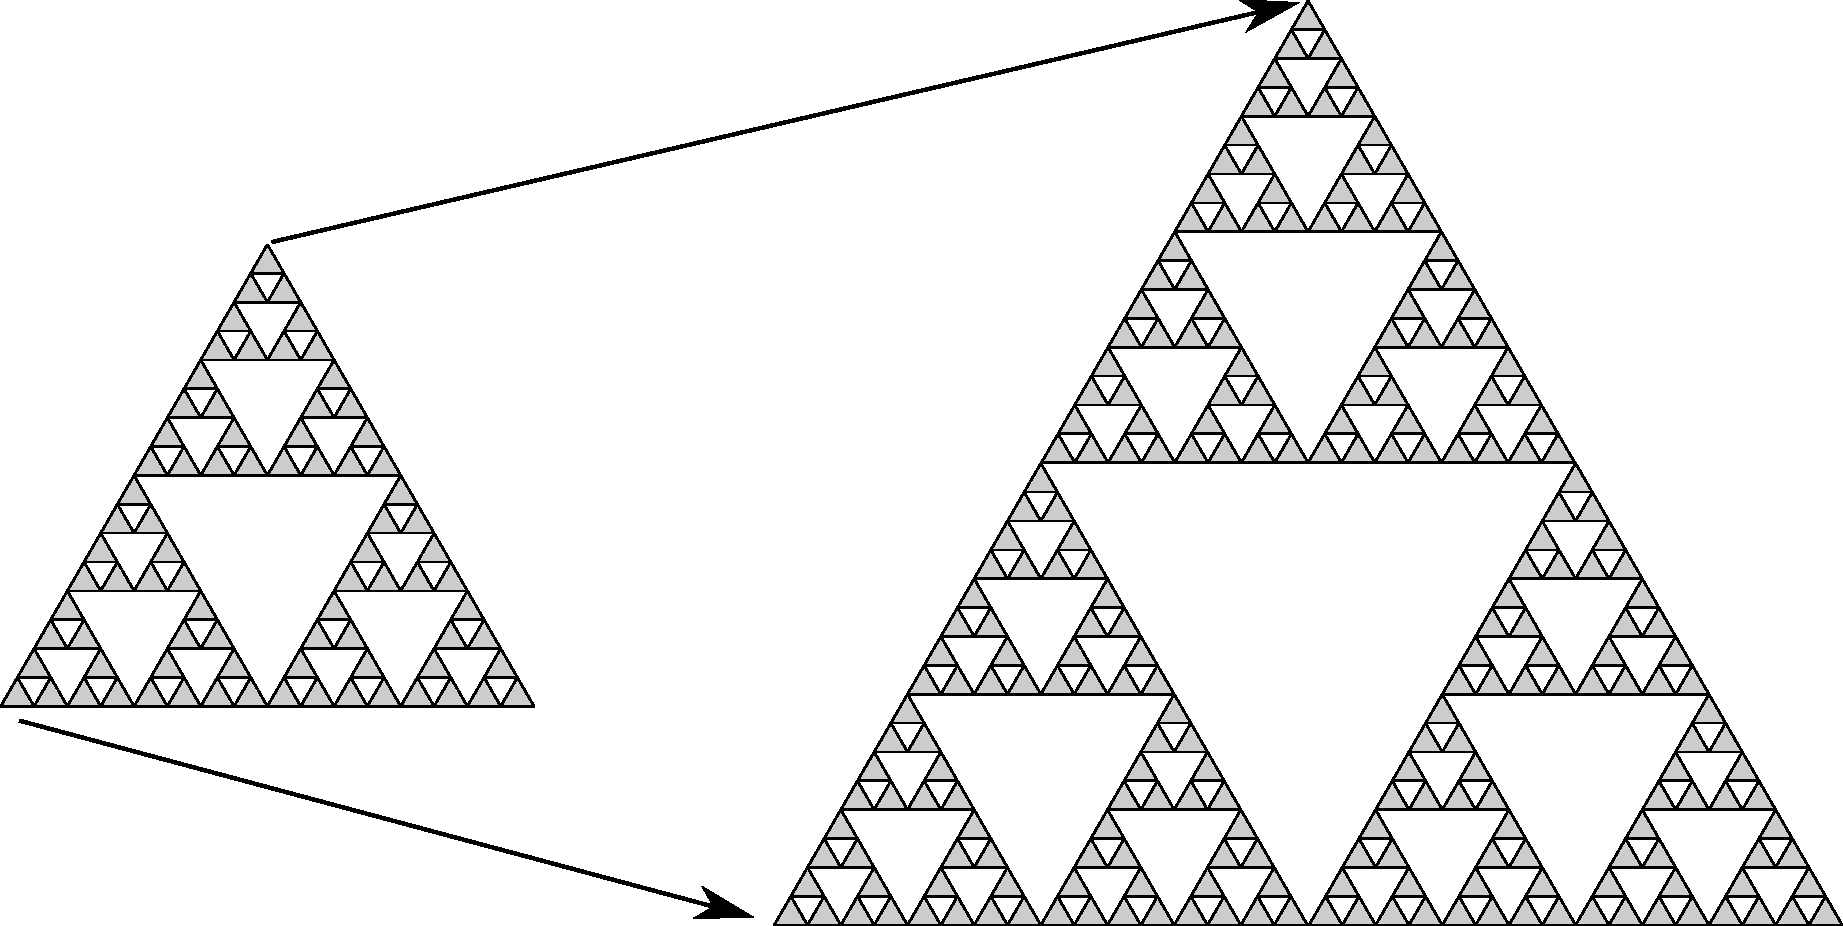
\includegraphics[width=.5\textwidth]{Bilder/Sierpinski-Dreieck-Vergroessern.pdf}
	\end{center}
	Streckst du das Sierpinski-Dreieck um den Faktor $2$, so passt das ursprüngliche Dreieck $3$-mal in das neue. Genau wie bei der letzten Aufgabe, liegt dessen Dimension also irgendwo zwischen $1$ und $2$. Genauer gesagt wiederum $d \approx 1,585$.
\end{aufgabe}

\begin{aufgabe}{}
	In jedem Schritt verliert man $\frac{1}{4}$ der grauen Fläche. Es bleiben also nach jedem Schritt $\frac{3}{4}$ der Fläche vor dem jeweiligen Schritt.
	
	Ist die Fläche des grauen Dreiecks zu Beginn $1$, so hat man nach einem Schritt eine Fläche von $\frac{3}{4}\cdot 1 = \frac{3}{4}$, nach zwei Schritten eine Fläche von $\frac{3}{4} \cdot \frac{3}{4} = \left(\frac{3}{4}\right)^2$ usw.
	
	Nach $n$ Schritten bleibt also noch eine Fläche von $\left(\frac{3}{4}\right)^n$. Man kann sich überlegen, dass der Flächeninhalt dadurch kleiner als jede positive Zahl wird. Folglich ist der Flächeninhalt des Fraktals (\glqq nach unendlich vielen Schritten\grqq) $0$.
\end{aufgabe}

\begin{aufgabe}{Pascalsches Dreieck}
	\begin{center}
		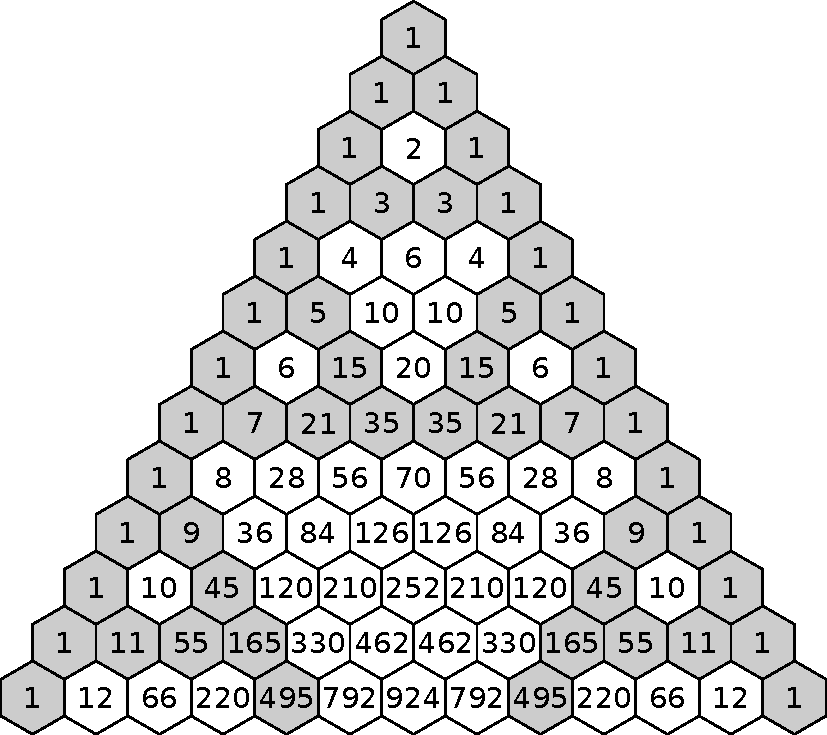
\includegraphics[width=.6\textwidth]{Bilder/Pascalsches-Dreieck-gefuellt-grau.pdf}
	\end{center}
\end{aufgabe}

\begin{aufgabe}{Cantor-Menge}
	Streckt man die Cantor-Menge um den Faktor $3$, so erhält man zwei Kopien des ursprünglichen Fraktals. Bei einer Strecke erhielte man drei Kopien. Die Cantor-Menge hat also eine \emph{kleinere} fraktale Dimension als die Strecke - also eine Dimension zwischen $0$ und $1$ - genauer: $d \approx 0,631$.
	
	Nach jedem Schritt hat die Strecke nur noch $\frac{2}{3}$ der vorherigen Länge. Nach $n$ Schritten also noch $\left(\frac{2}{3}\right)^n$. Und wie beim Sierpinski-Dreieck kann man sehen, dass diese Länge immer mehr gegen $0$ geht.
\end{aufgabe}

\begin{aufgabe}{Pyramiden-Fraktal}
	Bei jedem Schritt verfünffacht sich die Zahl der Pyramiden. Nach dem zweiten Schritt, haben wir also bereits $25$ Pyramiden.
	
	Streckt man das Pyramiden-Fraktal um den Faktor $2$, so erhält man $5$ Kopien. Ein Vergleich mit der Tabelle aus Aufgabe 3 zeigt also, dass die fraktale Dimension dieses Objekts zwischen $2$ und $3$ liegen muss. Genauer gesagt ist $d \approx 2,322$.
\end{aufgabe}
	
\begin{aufgabe}{}
	Das Pyramiden-Fraktal hat also eine Dimension zwischen $2$ und $3$. Ein solches Fraktal hatten wir bisher noch nicht gesehen, dafür aber gleich zwei mit einer Dimension zwischen $1$ und $2$: Die Kochsche Kurve und das Sierpinski-Dreieck. Bei der Kochschen Kurve haben wir bereits festgestellt, dass sie eine \emph{unendliche Länge} hat (und Länge ist eine Eigenschaft von \emph{ein}dimensionalen Objekten). Beim Sierpinski-Dreieck haben wir gezeigt, dass es eine \emph{Fläche von $0$} hat (und Fläche ist eine Eigenschaft von \emph{zwei}dimensionalen Objekten).
	
	Jetzt machen wir - etwas ungenau formuliert - \glqq alles eine Dimension höher\grqq: Wir haben ein Fraktal mit Dimension zwischen $2$ und $3$ und wollen dessen Fläche (Eigenschaft von \emph{zwei}dimensionalen Objekten) und dessen Volumen (Eigenschaft von \emph{drei}dimensionalen Objekten) bestimmen. Eine naheliegende Vermutung wäre daher, dass das Pyramiden-Fraktal eine unendliche Fläche, aber ein Volumen von $0$ hat.
	
	Tatsächlich kommt man auch auf das gleiche Ergebnis, wenn man wie zuvor überprüft, wie sich Fläche und Volumen bei jedem einzelnen Schritt verändern:
	Die Fläche ist nach einem Schritt $\frac{5}{4}$-mal so groß (wird also mehr) und das Volumen $\frac{5}{8}$-mal so groß (also kleiner). Auf diese Zahlen kommt man, wenn man sieht, dass aus einer einzelnen Pyramide in einem Schritt fünf Pyramiden werden, die halb so breit, halb so tief und halb so hoch sind.
\end{aufgabe}

\begin{aufgabe}{}
	Strecken wir dieses Möchtegern-Fraktal um den Faktor $2$, erhalten wir ein Objekt, dass aus $4 = 2^2$ Kopien des ursprünglichen besteht. Vergleichen wir das mit der Tabelle aus Aufgabe 3, sehen wir, dass das gerade zum Verhalten eines \emph{zweidimensionalen} Objektes passt. Anscheinend ist das hier also gar kein \glqq echtes Fraktal\grqq!
	
	\begin{center}
		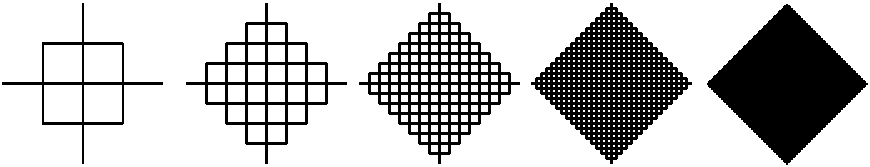
\includegraphics[width=.6\textwidth]{Bilder/Nicht-Fraktal-mehr-Schritte.pdf}
	\end{center}	
	
	Tatsächlich handelt es sich hierbei um eine sogenannte \glqq flächenfüllende\grqq{} Figur.\footnote{Die Bezeichnung \glqq flächenfüllen\grqq{} ist ein wenig irreführend, denn unsere Figur füllt die Fläche nicht wirklich komplett auf. In dem obigen Bild sieht das nur deshalb so aus, weil mein Computer keine unendlich dünnen Linien zeichnen kann. Allerdings liegen die einzelnen Linien, aus denen unsere Figur besteht, zumindest \glqq beliebig nahe aneinander\grqq{} und kommen jedem Punkt der überdeckten Fläche \glqq beliebig nahe (was gerade die mathematische Definition von \glqq flächenfüllend\grqq{} ist). Die Figur ist also im Grunde ein unendlich feines Gitter.} 
\end{aufgabe}

\begin{aufgabe}{Ostseeküste}
	Wie schon in Aufgabe 11 können wir folgende Vermutungen aufstellen:
	\begin{itemize}
		\item Eine fraktale Dimension $< 1$ führt zu einer Länge von $0$ (vgl. Cantor-Menge in Aufgabe 9).
		\item Eine fraktale Dimension $> 1$ führt zu einer Länge von unendlich (vgl. Kochsce Kurve).
		\item Eine (normale) Dimension $= 1$ sollte natürlich zu einer ganz normalen, endlichen Länge führen.
	\end{itemize}
	
	Beim tatsächlichen Messen der Küstenlänge stellt man fest, dass die Küste umso länger zu werden scheint, je genauer man misst (sprich: Je detaillierter die Karte ist, die man verwendet). Es sieht also so aus als wäre die Ostseeküste tatsächlich ein Fraktal der Dimension $> 1$.
\end{aufgabe}

\end{document}
